% \textit{\textbf{The following section formatting is \textbf{optional}, you can also define sections as you deem fit.
% \\
% Focus on what future researchers or practitioners would find useful for reproducing or building upon the paper you choose.\\
% For more information of our previous challenges, refer to the editorials \cite{Sinha:2022,Sinha:2021,Sinha:2020,Pineau:2019}.
% }}
\section{Introduction}
% A few sentences placing the work in high-level context. Limit it to a few paragraphs at most; your report is on reproducing a piece of work, you don’t have to motivate that work.
Recent work in the field of AI concerned with bias in machine learning has been focused on creating fair algorithms \cite{thomas2019preventing, agarwal2018reductions}. However, if demographic shifts occur within the data the model was trained on, such a model can often not maintain its fairness \cite{giguere2022fairness}. A demographic shift occurs when certain subgroups in a population are found more or less frequently in deployment. This can result in the model being biased towards certain groups, even if the model was originally trained to be equally fair to all groups \cite{schrouff2022maintaining}. It is therefore crucial to not only ensure the fairness of the model, but to also take into account possible shifts occurring after deployment. This encourages that the models are still making fair and accurate predictions in a possibly \textit{shifted} population.

To train models that are not only fair during training, but also have high-confidence fairness guarantees after deployment, \citeauthor{giguere2022fairness} introduce a new type of learning algorithm called \texttt{Shifty}. This algorithm ensures fairness after known and unknown demographic shifts in the data \cite{giguere2022fairness}. According to the authors, \texttt{Shifty} provides a high probability of the fairness constraints being met when deployed on data that is distributed differently, with respect to a demographic group, than it was during training. In the case of a known shift, the exact demographic shift is known, while with an unknown shift this is approximated by user-specified intervals. % not the case.

The main contributions of this work are:
\begin{itemize}
    \item Determining the degree of reproducibility, by recreating the main experiments conducted by \citeauthor{giguere2022fairness}, and concluding whether claims made in their research are factual, while considering what resources, such as computational power, are needed to come to this conclusion.
    
    \item Improving the efficiency and workings of the code by resolving errors, cleaning up the structure, and removing redundancies.
    % Miscchien overbodig 
    \item Examining the validity of the claims by introducing an unseen dataset with an unknown demographic shift. 
    
    \item As the authors mention that \texttt{Shifty} in practice works with any learning algorithm, the original research is expanded by using a different training algorithm than the one examined in the original paper.
\end{itemize}

\section{Scope of reproducibility}
% Introduce the specific setting or problem addressed in this work, and list the main claims from the original paper. Think of this as writing out the main contributions of the original paper. Each claim should be relatively concise; some papers may not clearly list their claims, and one must formulate them in terms of the presented experiments. (For those familiar, these claims are roughly the scientific hypotheses evaluated in the original work.)
\label{sec:claims}
The central claim introduced in this paper is that \texttt{Shifty} returns a machine learning algorithm that has a high probability of performing fair classification, before and after deployment, given a user-specified fairness constraint. This constraint is defined to maintain fairness concerning a sensitive attribute such as race or sex. Importantly, \texttt{Shifty} does not require access to the deployment data to ensure these guarantees. More specifically, the authors claim the following:
\begin{itemize}
    \item \textbf{High-confidence fairness guarantees:} In the case of a known or unknown demographic shift, \texttt{Shifty} provides high-confidence guarantees that a certain user-specified fairness constraint will hold even after the shift.
    
    \item \textbf{Minor loss of accuracy:} In the case of a known or unknown demographic shift, if enough data is provided, \texttt{Shifty} is able to train models, whose resulting accuracy is then comparable to that of models which do not account for demographic shift, such as \texttt{Fairness Constraints} \cite{zafar2017fairness} and \texttt{Seldonian} \cite{thomas2019preventing}. 
    
    \item \textbf{Finding a solution:} As the amount of training data increases, the probability of \texttt{Shifty} returning \verb|No Solution Found| (\verb|NSF|) decreases.

\end{itemize}

The remainder of this paper is structured as follows: In section \ref{sec:model_desc}, we give a detailed description of \texttt{Shifty} and the fairness algorithms it was compared to. In section \ref{sec:method}, the methods that were used to verify the claims of the authors are set out. This includes an explanation of the datasets, the hyperparameters, the experimental setup and code, and lastly the computational requirements needed to come to the results. Moreover, we elaborate on the steps taken to conduct additional research. Then, the results of this study are discussed and compared to the original results in section \ref{sec:results}. Finally, we conclude this study by discussing and evaluating the used approach.


\section{Model descriptions}
\label{sec:model_desc}
% Include a description of each model or algorithm used. Be sure to list the type of model, the number of parameters, and other relevant info (e.g. if it's pretrained). 

\subsection{\texttt{Shifty}}
The \texttt{Shifty} algorithm is made up of three main parts of which a short overview is given below and which are later discussed more elaborately:
\begin{enumerate}
    \item The first step consists of partitioning the dataset $D = \{(X_i,Y_i,S_i,T_i)\}^n_{i=1}$ into two parts. Each sample in $D$ is uniformly distributed and consists of a feature, label, fairness attribute, and demographic attribute respectively. One part of $D$ is used for candidate model selection, called $D_c$ and the other is used to perform a fairness test, called $D_f$. 

    \item Secondly, the candidate model, denoted as $\theta_c$, is trained using $D_c$, which can be any classification model, while a user-specified fairness constraint is taken into account, also denoted by a function of $g$. During training, the features, labels, and fairness attributes are used. The candidate model is deemed fair if $g(\theta_c) \leq 0$. This is calculated by inverting Student's \textit{t}-test \cite{student} and is given by Equation \ref{eq:inverse_ttest}, where $\mathbf{E}[H|\xi]-\tau= g(\theta_c)$.

    \item Lastly, a high-confidence upper bound (HCUB) on the candidate model is calculated after it is deployed in an environment affected by a demographic shift, which is simulated using the demographic attribute. $g'(\theta_c)$ denotes the fairness of $\theta_c$ after deployment and should also be less or equal to zero with high confidence, which then again is calculated using the inverted \textit{t}-test.
    
\end{enumerate}

For the third step, the description of the possible demographic shifts is defined by $\mathcal{Q}:=\{ (a_t,b_t) \}_{t\in\mathcal{T}}$. It is a user-defined set of upper and lower boundaries on the marginal probability of each demographic attribute value after deployment. If the demographic shift is known then $\forall_{t\in\mathcal{T}}[a_t = b_t = Pr(T'=t)]$, where $Pr(T'=t)$ is the probability of demographic attribute $t$ occurring after deployment. 

\vspace{-1.5em}
\begin{align}
\label{eq:inverse_ttest}
    Pr(\mathbf{E}[H|\xi] \leq U_{ttest}(g, D,\theta,\delta))\geq 1-\delta \text{, where $\delta \in [0,1]$}
\end{align}

% \vspace{-2em}
% \begin{align}
% \label{eq:inverse_ttest}
%     Pr(\mathbf{E}[\hat{H}|\xi] \leq \hat{U}_{ttest}(g, D,\theta,\delta)) = Pr(\mathbf{E}[H'|\xi'] \leq \hat{U}_{ttest}(g, D,\theta,\delta)) \geq 1-\delta
% \end{align}

% Given a dataset $D$, a description of a demographic shift $\mathcal{Q}$, and one or more fairness specifications, the \texttt{Shifty} algorithm returns a model with a high-confidence fairness guarantee. 
% A fairness specification consists of a function $g$ to assess the fairness of a model given a specific constraint, and a confidence bound $\delta$. According to \citeauthor{giguere2022fairness}, a training algorithm $a$ is guaranteed to be fair if Equation \ref{eq:gauranteefairness} holds for an algorithm $a$ and a dataset $D$. The first step of \texttt{Shifty} is splitting the training data into two different partitions, $D_c$ and $D_f$, which are used for candidate selection and fairness testing, respectively. 

% The $D_c$ partition is first used to train a linear classification model $\theta_c$ that produces the smallest classification loss. This model $\theta_c$ is equivalent to the $a(D))$ in Equation \ref{eq:gauranteefairness}. 

% Then, the $D_f$ partition of the data and the description of the demographic shift $\mathcal{Q}$ are used to calculate the $(1 - \delta)$-confidence upper bound (HCUB) on the $g(\theta_c)$, for each fairness specification to observe whether the candidate model $\theta_c$ is fair during deployment or not. If the HCUB is below 0, \texttt{Shifty} returns the model $\theta_c$ with fairness guarantee after demographic shift. If this HCUB is equal to or greater than zero, no fair candidate model is found and \texttt{Shifty} returns \texttt{No Solution Found} (NSF). The probability as seen in Equation \ref{eq:gauranteefairness} is calculated by counting how often \texttt{Shifty} accepts a model as a fair model over multiple trials, whilst $g > 0$, so the model is actually unfair after deployment. This is used to compute the standard error and whether the resulting number is smaller than $\delta$ the high-confidence fairness guarantee of \ref{eq:gauranteefairness} holds, otherwise it does not.
% - over de 10 trials kijken hoevaak seldonian model accept terwijl g>0 en hierover standard error berekenen. is dit hoger dan delta? dan voldoet shifty niet aan die high-confidence, maar dit is nooit het geval :)

\subsection{Baselines} \label{sec:baselines}
To assess \texttt{Shifty}'s effectiveness, it was compared to other algorithms, namely \texttt{Fairness Constraints} \cite{zafar2017fairness}, \texttt{Seldonian}, \texttt{Quasi-Seldonian} \cite{thomas2019preventing}, \texttt{Fairlearn} \cite{agarwal2018reductions}, and \texttt{RFLearn} \cite{du2021fair}. The features of these algorithms are summarized in Table \ref{tab:algorithms}. Of these algorithms, \texttt{Shifty} is thus the first algorithm to provide fairness guarantees under demographic shift.

\begin{table}[ht]
    \centering
    \footnotesize
    \begin{tabular}{c|c|c}
       Algorithm & Classifier & Difference with Shifty\\\hline
       FC & Decision boundary & Does not account for demographic shift\\
       Seldonian & Linear decision boundary & Does not account for demographic shift\\
       Q-Seldonian & Linear decision boundary & Does not account for demographic shift\\
       Fairlearn & Linear SVC & Does not account for demographic shift\\
       RFLearn & Logistic regression & Does not provide fairness guarantees\\
    \end{tabular}
    \caption{\textbf{Algorithms overview.} For each algorithm, its classifier and its difference with \texttt{Shifty} are specified. `FC' stands for \texttt{Fairness Constraints} and `Q-Seldionian' is the \texttt{Quasi-Seldonian} algorithm.}
    \label{tab:algorithms}
\end{table}

% Fairness Constraints uses a classifier with a decision boundary, but does not provide fairness without guarantees. Both the Seldonian and Quasi-Seldonian algorithms use a linear classifier and provide high-confidence fairness guarantees for a user-specified fairness definition, but do not account for demographic shift. Fairlearn uses a linear support vector classifier and provides high-confidence fairness guarantees while also not accounting for demographic shifts. Finally, RFLearn promotes fairness under covariant shift, but does not provide any fairness guarantees.

\subsection{Fairness Constraints}
The fairness constraints that \texttt{Shifty} uses are user-specified. In this study and in the original paper, two fairness constraints are utilized, namely Demographic Parity (DP) and Disparate Impact (DI). Equations \ref{eq:DP} and \ref{eq:DI} show the definitions of DP and DI, respectively. In these equations, $g$ represents the function to define unfair behaviour, $\theta(X)$ the model, $\epsilon$ the fairness constraint tolerance hyperparameter, and $S$ the sensitive fairness attribute. In the case of $S$ being the attribute \texttt{sex}, $s_0$ and $s_1$ would represent \texttt{male} and \texttt{female}.
\vspace{-1.5em}
\begin{align}\label{eq:DP}
\footnotesize
    g_{DP} := |\mathbb{E}[\theta(X)|S=s_0] - \mathbb{E}[\theta(X)|S=s_1]| - \epsilon_{DP}
\end{align}

\vspace{-1.5em} % deze doet vgm niks :(
% Zirk: Dan met je er \vspace*{-1.5em} van maken
\begin{align}\label{eq:DI}
\footnotesize
    g_{DI} := - \min(\frac{\mathbb{E}[\theta(X)|S=s_0]}{\mathbb{E}[\theta(X)|S=s_1]}, \frac{\mathbb{E}[\theta(X)|S=s_1]}{\mathbb{E}[\theta(X)|S=s_0]}) + \epsilon_{DI}
\end{align}

\section{Methodology} \label{sec:method}
% Explain your approach - did you use the author's code, or did you aim to re-implement the approach from the description in the paper? Summarize the resources (code, documentation, GPUs) that you used.
We reproduced the original results from the paper using the open-source implementation of the code as provided by the authors on GitHub \cite{giguereGithub}. This code was analyzed to understand how the results were achieved. The provided code is partly based on the papers that cover the different fairness algorithms that \texttt{Shifty} is compared to (section \ref{sec:baselines}). A code coverage analysis revealed that a large fraction of the code was not used to obtain the results corresponding to the experiments as discussed in the paper. 


\subsection{Datasets}\label{sec:datasets}
% What the format says should be in this section
% For each dataset include 1) relevant statistics such as the number of examples and label distributions, 2) details of train / dev / test splits, 3) an explanation of any preprocessing done, and 4) a link to download the data (if available).
To verify the results, this reproducibility study used the same data to conduct the experiments. The authors provided the pre-processed datasets and the code to pre-process the original data. This pre-processing resulted in datasets with zero mean and unit variance. For the non-Seldonian algorithms, both datasets were split up into a 6:4 ratio of train and test data. For the Seldonian algorithms, the ratio was a 6:4 of data for the candidate selection ($D_c$) and fairness testing ($D_f$) subsets. 

The original paper conducted experiments on the \textit{UCI Adult Census} dataset \cite{adult_dataset} and the \textit{UFRGS Entrance Exam and GPA} dataset \cite{gpa_dataset}. To further validate the claims made by the authors, an additional dataset was acquired containing approximately 50k diabetic patient encounters collected over a period of 10 years from 130 US hospitals \cite{strack2014impact}. This dataset will subsequently be referred to as \textit{Diabetes}. Each encounter recorded several statistics to help determine the relationship between the probability of readmission and hbA1c measurement depending on primary diagnosis. For all datasets, we present the relevant statistics and their main purpose in Table \ref{tab:datasets}.

\begin{table}[ht]
    \centering
    \footnotesize
    \begin{tabular}{c|c|c|c|c}
       Datasets & Task & Samples & Fairness attr. & Demographic attr. \\\hline
       UCI Adult Census \cite{adult_dataset} & Predict income above \$50k & 43k & Race & Sex \\
       UFRGS \cite{gpa_dataset} & Predict GPA above 3.0 & 43k & Sex & Race \\ 
       \multirow{2}{*}{Diabetes \cite{strack2014impact}} & \multirow{2}{*}{Predict readmission} & 47k & Race & Sex \\
       & & 49k & Sex & Race \\% multirow 
    \end{tabular}
    \caption{\textbf{Datasets overview.} All three datasets were used for binary classification tasks. In the \textit{UCI Adult Census} and \textit{Diabetes} datasets, the samples were filtered down to only include white and black individuals, when race is considered the fairness attribute.}
    \label{tab:datasets}
\end{table}

% The dataset used was the \textit{UCI Adult Census} dataset \cite{adult_dataset}, which describes various statistical features about a population, including race and sex. The dataset contains information about 48.842 individuals during the 1994 US census. The experiments used a subset of the dataset containing only black or white individuals, which resulted in 43.131 samples. This subset was used to classify whether an individual earns above or under \$50,000 each year. When testing the fairness of a trained model, the predictions were assessed using \texttt{sex} as the fairness attribute. \texttt{race} was used as the attribute to simulate a demographic shift, so it is referred to as the demographic attribute. 

% The original experiments used a second dataset, the \textit{UFRGS Entrance Exam and GPA} dataset \cite{gpa_dataset}, from which the results were not discussed. Hence, we chose to describe this dataset in the Appendix.
% The fairness is assessed by defining sex as the attribute that is used to evaluate fairness (fairness attribute), and race as the attribute where the demographic shift occurs (demographic attribute). 

%The second dataset used is the \textit{UFRGS Entrance Exam and GPA} dataset \cite{gpa_dataset}, which describes the academic records of 43.303 students from the Federal University of Rio Grande do Sul in Brazil. The dataset includes a vector of entrance exam scores for every student, a binary label representing if the student's GPA (on a scale from 0 to 4.0) was above or below 3.0, and labels for the student's race and sex, where now race is used as the fairness attribute, and sex as the demographic attribute.


\subsection{Hyperparameters}
% Describe how the hyperparameter values were set. If there was a hyperparameter search done, be sure to include the range of hyperparameters searched over, the method used to search (e.g. manual search, random search, Bayesian optimization, etc.), and the best hyperparameters found. Include the number of total experiments (e.g. hyperparameter trials). You can also include all results from that search (not just the best-found results).
The original authors' code included a batch file to run the experiments with specified hyperparameters (shown in Table \ref{tab:Adulthyperparams} for the \textit{UCI Adult Census} dataset; for \textit{UFRGS} results, see Appendix \ref{sec:appendix}). The provided code contained pre-determined values for the fairness constraint tolerance hyperparameter $\epsilon$ (used in equations \ref{eq:DP} and \ref{eq:DI}). It also provided the split ratio for training data and test data, and the split ratio for candidate data and fairness data for the Seldonian algorithms. The batch file also included the number of iterations considered for the training algorithm $a$, and the confidence bound $\delta$ (Eq. \ref{eq:inverse_ttest}). Lastly, for the unknown distributional shift the width of the intervals around true marginals representing the valid demographic shifts is given by an $\alpha$-value. 

\begin{table}[ht]
\centering
\footnotesize
    \begin{tabular}{l|c|c|c|c|c|c}
    Constraint & $\epsilon$ & train / test & Dc / Df & n-iters & $\delta$ & $\alpha$* \\\hline 
    DI & -0.8 & 0.4 & 0.4 &  2000 & 0.05 & 0.5\\
    DP & 0.1 & 0.4 & 0.4 & 2000 & 0.05 & 0.5 \\
    \end{tabular}
    \caption{Hyperparameter values for the experiments run with the \textit{UCI Adult Census} dataset specified for DI or DP for both an unknown demographic shift and a known demographic shift. The $\alpha$ is only used in the case of an unknown shift.}
    \label{tab:Adulthyperparams}
\end{table}

\subsection{Experimental setup and code} \label{sec:experiments}
% Include a description of how the experiments were set up that's clear enough a reader could replicate the setup. 
% Include a description of the specific measure used to evaluate the experiments (e.g. accuracy, precision@K, BLEU score, etc.). 
% Provide a link to your code.
In the original experiments, each algorithm was trained with different-sized subsets of the data to determine how much data was needed to maintain a fairness guarantee under demographic shift. For a known demographic shift, we used subset sizes ranging from 10k to 60k points, in intervals of 5k datapoints. For an unknown demographic shift, we increased the intervals to 10k while the range remained the same. In a single trial for an user-specified constraint, the results per subset size were collected for each algorithm for both cases of a known and unknown demographic shift.

The original paper specified that 25 trials were executed for each fairness constraint in both cases of a known or unknown demographic shift and for each dataset mentioned in section \ref{sec:datasets}. In our experiments, due to a lack of computational resources, we only executed 10 trials for each case.

The original classifier that we used for the three Seldonian algorithms was a linear decision boundary. Additionally, we implemented a multi-layer perceptron (MLP) as a classification model that works with the Seldonian algorithms. The preferred classifier and the sizes of the hidden layers can be specified within the batch file and we used an MLP with 2 hidden layers of sizes 16 and 8. Furthermore, we instantiated the weight parameters according to the normal distribution and optimized these in the same way as the original \texttt{Shifty} implementation. This experiment was run for 2 trials for each constraint mentioned previously, for a known and unknown demographic shift. 

After every single trial, we saved the results for each algorithm and subset size. These results contained the probability of a \verb|NSF|, the accuracy of the original model and the accuracy of the deployed model, as well as the failure rate of the original model and the failure rate of the deployed model. After completing all the trials, the mean and standard error were determined for each of these measurements. The code of this reproducibility study can be found \href{https://anonymous.4open.science/r/fact_guarantee-DB57/}{here}.
% \href{https://github.com/noanonkes/fact_ai_group7/tree/clean}{here}.

\subsection{Computational requirements}
% Include a description of the hardware used, such as the GPU or CPU the experiments were run on. 
% For each model, include a measure of the average runtime (e.g. average time to predict labels for a given validation set with a particular batch size).
% For each experiment, include the total computational requirements (e.g. the total GPU hours spent).
% (Note: you'll likely have to record this as you run your experiments, so it's better to think about it ahead of time). Generally, consider the perspective of a reader who wants to use the approach described in the paper --- list what they would find useful.
The code provided by the original authors contains an elaborate launcher that allows the experiments to be run with CPU multiprocessing. The CPU used to obtain the results was an \textit{AMD Ryzen 7 3800X} processor, utilizing 8 cores simultaneously. 

During the process, the time required per trial was recorded. This was done for each dataset, as well as for each constraint for both the known and unknown demographic shift. These times were then averaged. For the \textit{UFRGS} dataset this resulted in 15.5 minutes per trial, while the \textit{UCI Adult Census} dataset resulted in 24 minutes per trial. The total (CPU) time required, resulted in 26 hours for the reproduction of the original experiments. The additional experiments entail 28 additional hours for the experiments run with the \textit{Diabetes} dataset, and 60 hours for the experiments run with MLP classifier, concluding to roughly 115 hours total needed for the considered experiments.

\section{Results} 
\label{sec:results}
% Start with a high-level overview of your results. Do your results support the main claims of the original paper? Keep this section as factual and precise as possible, reserve your judgement and discussion points for the next "Discussion" section. 
% Section \ref{sec:claims} describes the three main claims that were made in the original paper. 
In this section, we discuss the reproduction results from the original paper and the results from the additional experiments. To verify the claims set out in section \ref{sec:claims}, the experiments were executed as described in section \ref{sec:experiments}. The results of these experiments include the probabilities that the Seldonian algorithms return \texttt{NSF}, and the accuracies and failure rates of the algorithms before and after deployment.
The graphs of these results show the means and standard errors. The resulting accuracies and failure rates of the models can be found in Appendix \ref{sec:failure_rates_appendix} \& \ref{sec:app_num_results}.

The two fairness constraints, DP and DI, were examined for both datasets. As in the original paper, only the reproduced results of the \textit{UCI Adult Census} dataset are shown. The results of the \textit{UFRGS} dataset can be found in Appendix \ref{sec:appendix1}.


\subsection{Results reproducing original paper} \label{sec:originalresults}
% For each experiment, say 1) which claim in Section~\ref{sec:claims} it supports, and 2) if it successfully reproduced the associated experiment in the original paper. 
% For example, an experiment training and evaluating a model on a dataset may support a claim that that model outperforms some baseline.
% Logically group related results into sections. 
 
The following section showcases the results of the experiments as discussed in section \ref{sec:experiments}. In the sections \ref{sec:results1}, and \ref{sec:results2} the specific results for the known and unknown demographic shift are considered, respectively. %In section \ref{sec:additionalresults}, the results of additional experiments with the Seldonian classifiers using the MLP are shown. 

\subsubsection{Result 1: Known Demographic Shift}\label{sec:results1}
Figure \ref{fig:adult_known_shift} plots the probability that the \texttt{Seldonian}, the \texttt{Quasi-Seldonian}, and \texttt{Shifty} algorithms return \texttt{NSF} for a known demographic shift for the fairness constraints DP and DI, per data subset size.

\begin{figure}[ht]
    \begin{subfigure}{0.5\linewidth}
      \centering
      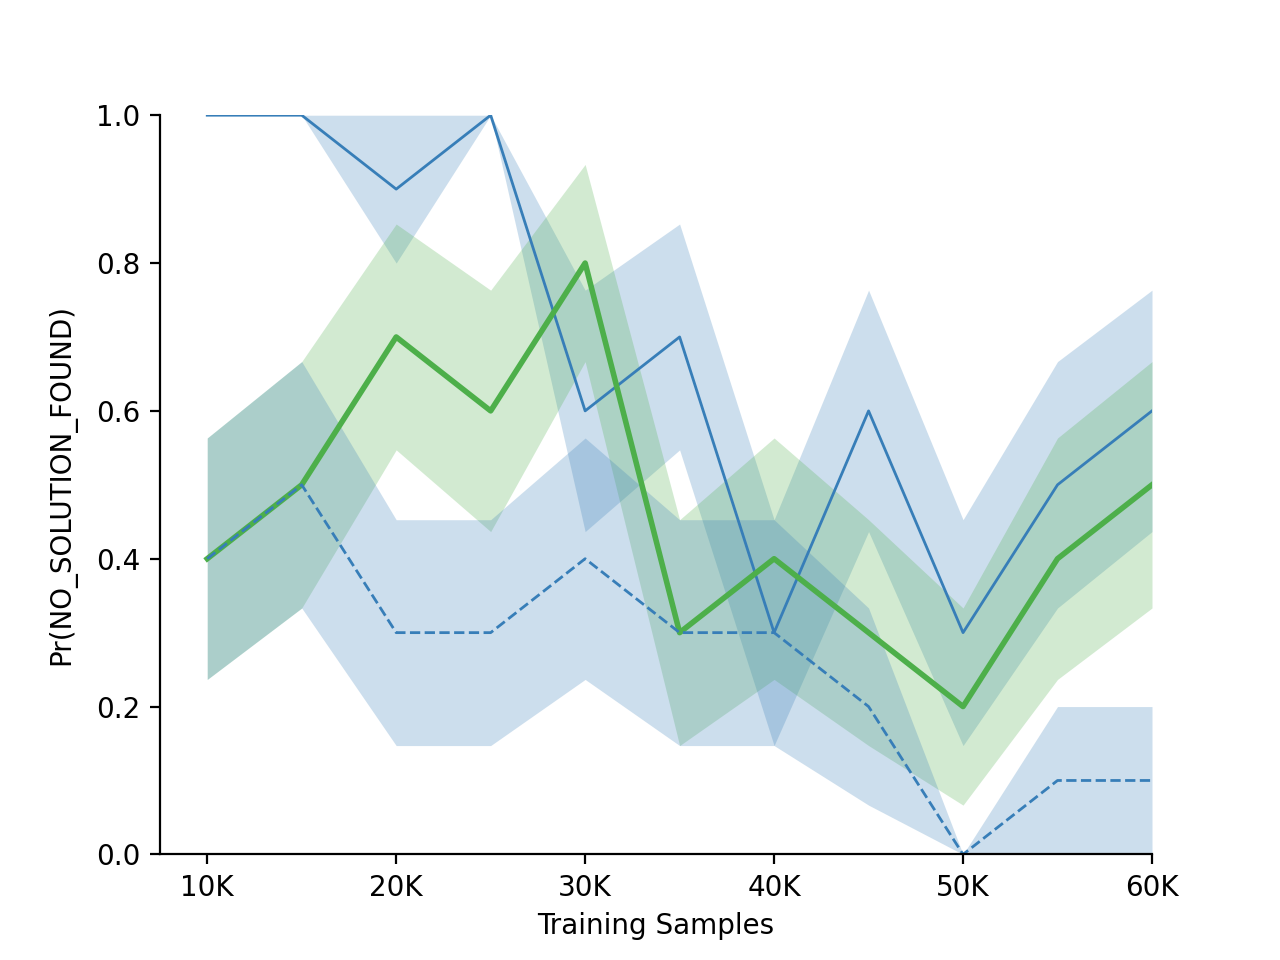
\includegraphics[width=0.8\linewidth]{figures/iclr_fixed_demographic_shift_adult_rl/iclr_adult_fixed_ds_rl_dp.png}
      \caption{Demographic Parity}
      \label{fig:adult_k_dp}
    \end{subfigure}
    \begin{subfigure}{0.5\linewidth}
      \centering
      \includegraphics[width=0.8\linewidth]{figures/iclr_fixed_demographic_shift_adult_rl/iclr_adult_fixed_ds_rl_di.png}
      \caption{Disparate Impact}
      \label{fig:adult_k_di}
    \end{subfigure}
    \begin{subfigure}{\textwidth}
    \includegraphics[width=\linewidth]{figures/iclr_legend.png}
    \end{subfigure}
    \caption{Probabilities of returning \texttt{NSF} per number of training samples when enforcing fairness constraints DP and DI using the \textit{UCI Adult Census} dataset under known demographic shift.}
    \label{fig:adult_known_shift}
\end{figure}

\subsubsection{Result 2: Unknown Demographic Shift}\label{sec:results2}
Figure \ref{fig:adult_unknown_shift} plots the probability that the \texttt{Seldonian}, the \texttt{Quasi-Seldonian}, and \texttt{Shifty} algorithms return \texttt{NSF} for an unknown demographic shift for the fairness constraints DP and DI, per data subset size.

\begin{figure}[ht]
    \begin{subfigure}{0.5\linewidth}
      \centering
      \includegraphics[width=0.8\linewidth]{figures/iclr_antag_demographic_shift_adult_rl/iclr_adult_antag_ds_rl_dp.png}
      \caption{Demographic Parity}
      \label{fig:adult_unk_dp}
    \end{subfigure}
    \begin{subfigure}{0.5\linewidth}
      \centering
      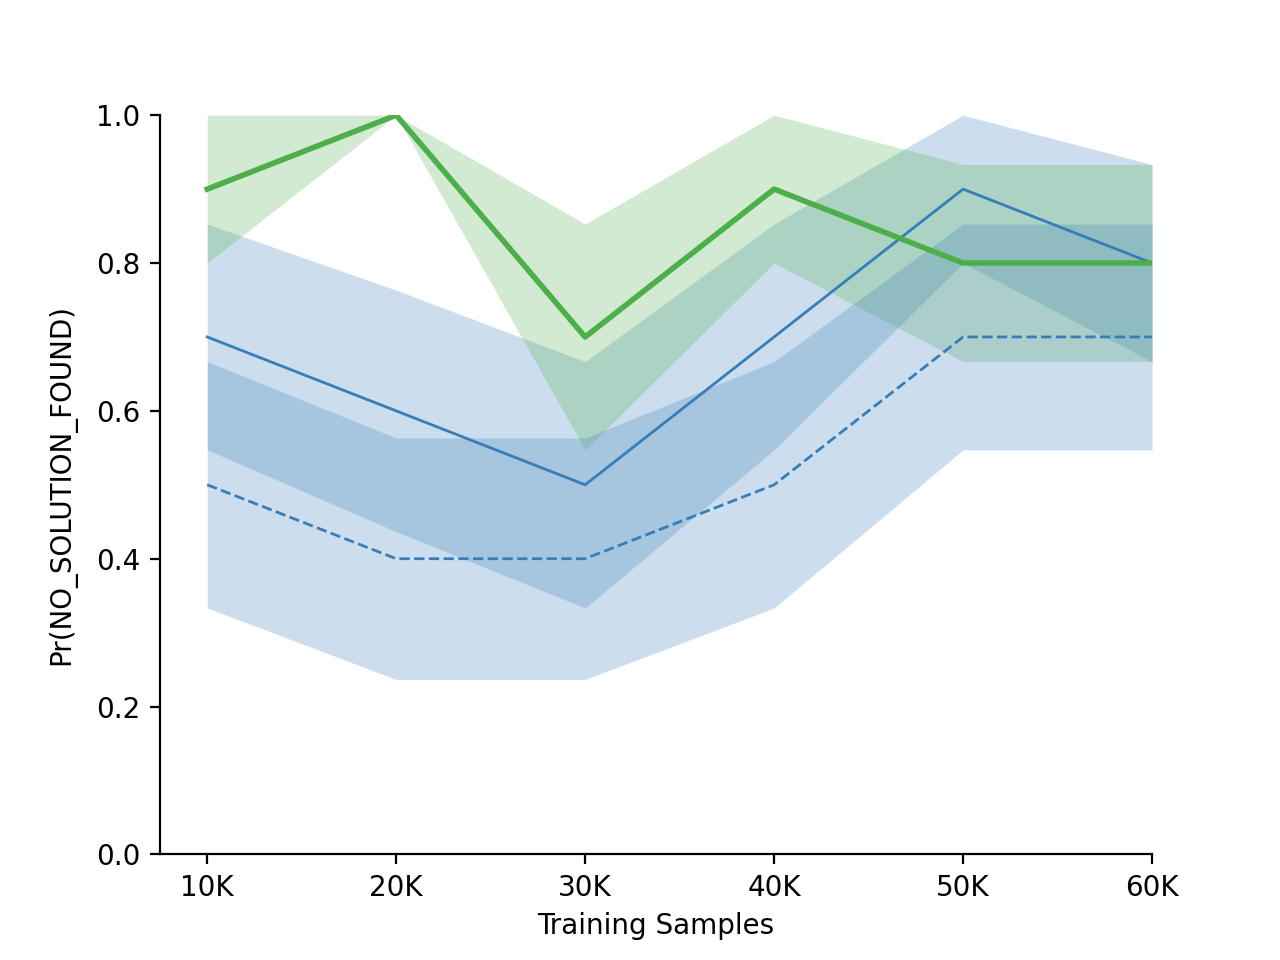
\includegraphics[width=0.8\linewidth]{figures/iclr_antag_demographic_shift_adult_rl/iclr_adult_antag_ds_rl_di.png}
      \caption{Disparate Impact}
      \label{fig:adult_unk_di}
    \end{subfigure}
    \begin{subfigure}{\textwidth}
        \includegraphics[width=\linewidth]{figures/iclr_legend.png}
    \end{subfigure}
    \caption{Probabilities of returning \texttt{NSF} per number of training samples when enforcing fairness constraints DP and DI using the \textit{UCI Adult Census} dataset under unknown demographic shift. }
    \label{fig:adult_unknown_shift}
\end{figure}


\subsection{Results beyond original paper} \label{sec:additionalresults}
% Often papers don't include enough information to fully specify their experiments, so some additional experimentation may be necessary. For example, it might be the case that batch size was not specified, and so different batch sizes need to be evaluated to reproduce the original results. Include the results of any additional experiments here. Note: this won't be necessary for all reproductions.
Additional experiments were conducted using a different dataset to substantiate the claims made by the authors. Further experiments were carried out to validate whether \texttt{Shifty} is successful independent of the classifier used. In the following section additional results will be discussed, using the \textit{Diabetes} dataset as specified in section \ref{sec:datasets} and the MLP classifier as specified in section \ref{sec:experiments}. 

\subsubsection{Additional Results 1}
Using the \textit{Diabetes} dataset, Figure \ref{fig:diabetes_unknown_shift} shows the probability that the \texttt{Seldonian}, the \texttt{Quasi-Seldonian}, and \texttt{Shifty} algorithms return \texttt{NSF} for an unknown demographic shift under the fairness constraint DI, per data subset size. In the left plot \textit{race} is considered the demographic attribute, and in the right plot \textit{sex} is considered the demographic attribute. 

\begin{figure}[ht]
    \begin{subfigure}{0.5\linewidth}
      \centering
      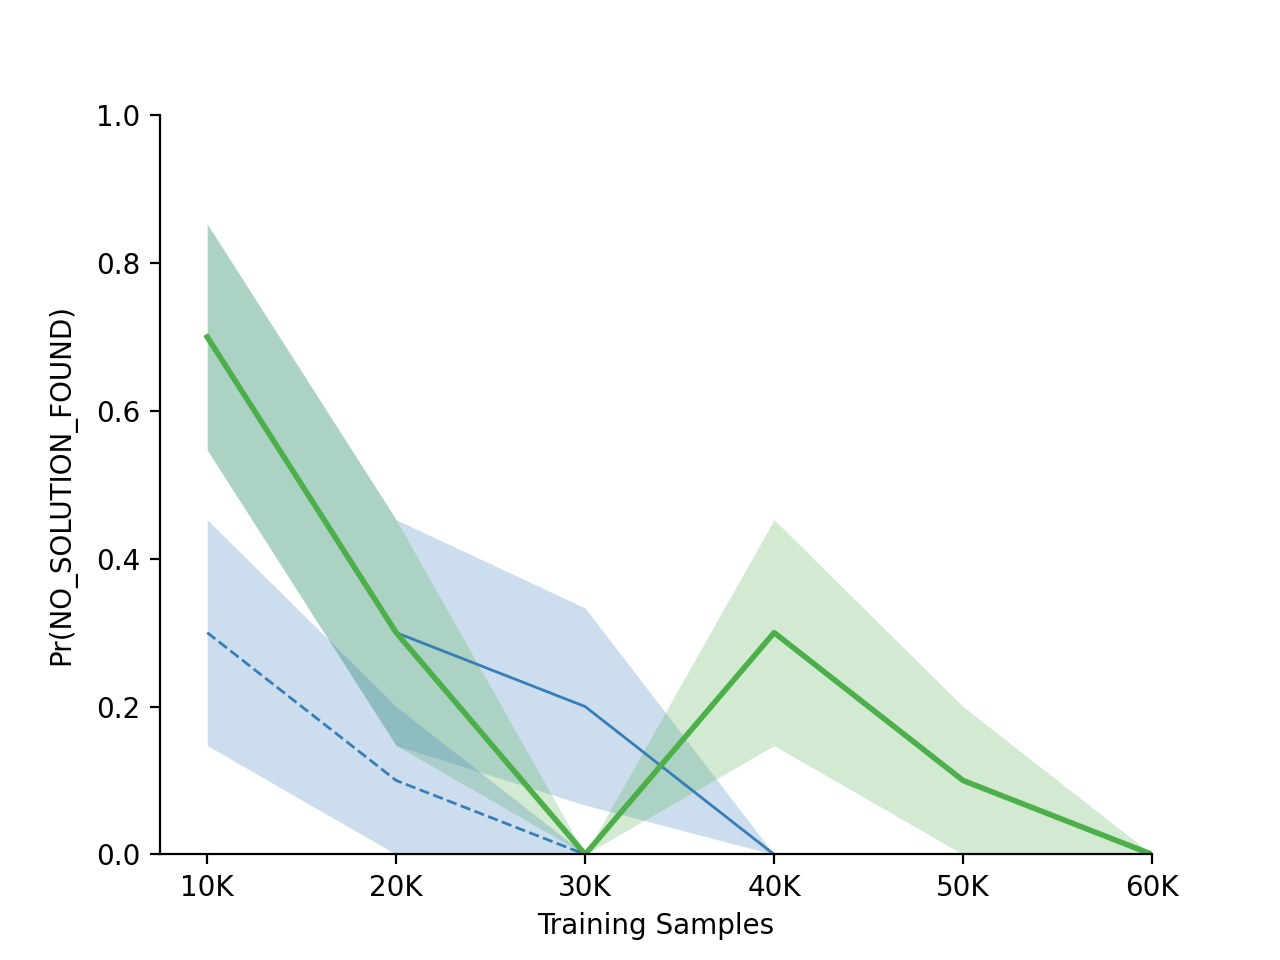
\includegraphics[width=0.8\linewidth]{figures/diabetes_P(NSF)/icrl_diabetes_antag_ds_rl_sex_di_P(NSF).png}
      \caption{Sex as demographic variable}
      \label{fig:diabetes_unknown_shift_sex}
    \end{subfigure}
    \begin{subfigure}{0.5\linewidth}
      \centering
      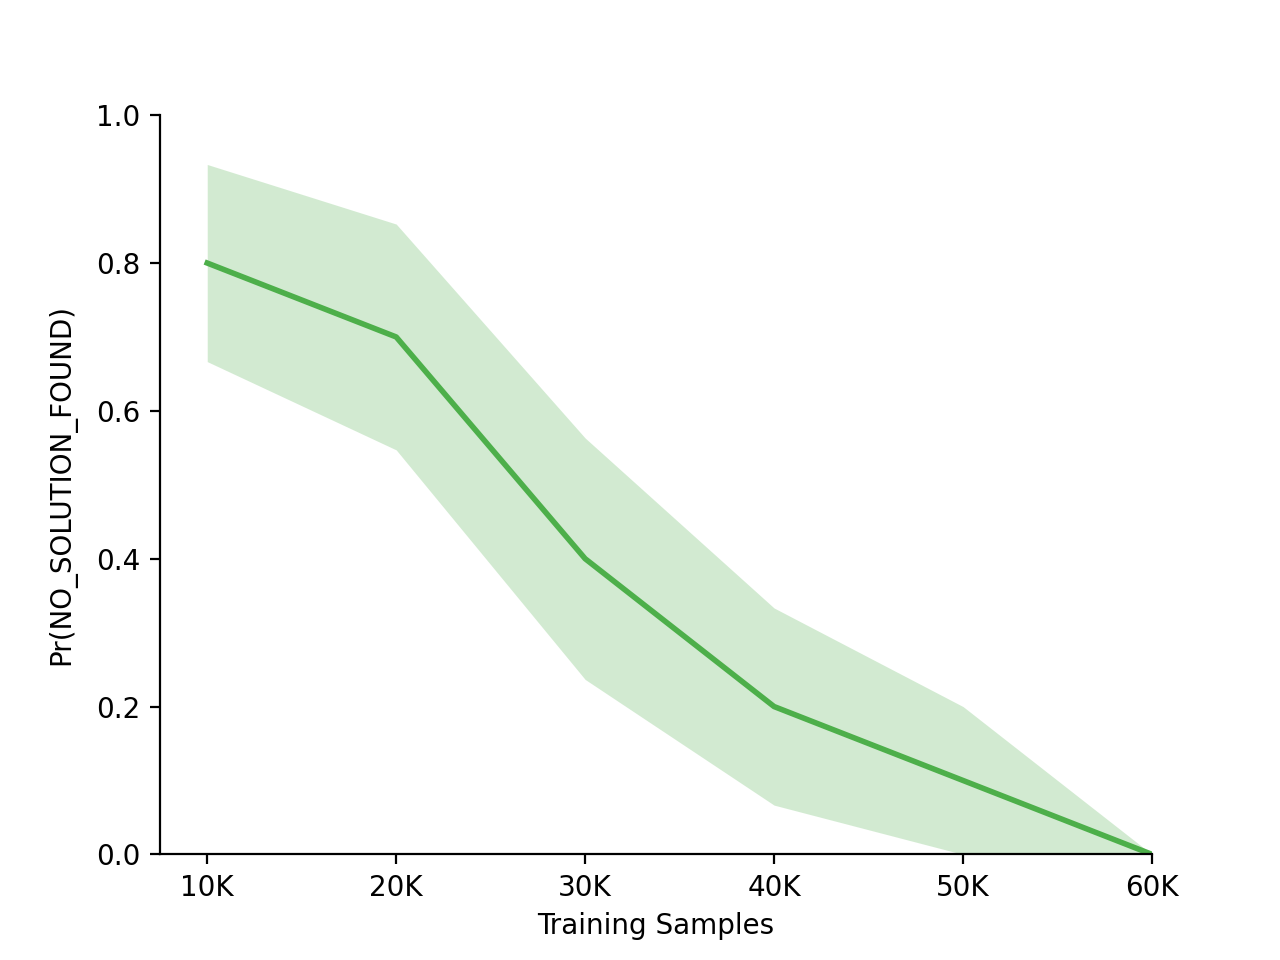
\includegraphics[width=0.8\linewidth]{figures/diabetes_P(NSF)/icrl_diabetes_antag_ds_rl_race_di_P(NSF).png}
      \caption{Race as demographic variable}
      \label{fig:diabetes_unknown_shift_race}
    \end{subfigure}
    \begin{subfigure}{\textwidth}
        \includegraphics[width=\linewidth]{figures/iclr_legend.png}
    \end{subfigure}
    \caption{Results when enforcing fairness constraint DI using the \textit{Diabetes} dataset under unknown demographic shift, with either the \textit{sex} or \textit{race} as demographic attribute. 
    }
    \label{fig:diabetes_unknown_shift}
\end{figure}



\subsubsection{Additional Result 2}
For the experiments run with an MLP classifier, the accuracies of the \texttt{Seldonian}, the \texttt{Quasi-Seldonian}, and \texttt{Shifty} algorithms are shown before and after deployment in Table \ref{tab:add_results}, using the \textit{UCI Adult Census} dataset. In case the algorithm was not able to return a fair model in any trial, the results show a \texttt{NaN}-value.


../openreview/tables.tex


\section{Discussion}
% Give your judgement on if your experimental results support the claims of the paper. Discuss the strengths and weaknesses of your approach - perhaps you didn't have time to run all the experiments, or perhaps you did additional experiments that further strengthened the claims in the paper.

\subsection{Claim 1: High-confidence fairness guarantees} \label{sec:discussion_fail}
The results found in this reproducibility study validate the first claim made by the original authors, which asserts the high-confidence fairness guarantee of \texttt{Shifty}. The \texttt{Shifty} algorithm never returns an unfair model after deployment for both a known and an unknown demographic shift, while other baseline algorithms do. The figures portraying the results of the reproduction experiments supporting this claim can be found in section \ref{sec:failure_rates_appendix} of the appendix.


\subsection{Claim 2: Minor loss of accuracy} \label{sec:discussion_accuracy}
The results found in this reproducibility study show strong support for the second claim made by the original authors, namely that there is only a minor loss of accuracy with \texttt{Shifty} when compared to the other baseline algorithms. This is the case under both a known and an unknown demographic shift, which can be seen in tables \ref{tab:uci_num_k_DP}, \ref{tab:uci_num_k_DI}, \ref{tab:uci_num_unk_DP}, and \ref{tab:uci_num_unk_DI} in the appendix section \ref{sec:app_num_results}. 

What does stand out is that in the case of DI as the fairness constraint and under a known demographic shift, \texttt{Shifty} achieves an accuracy that is approximately 10\% lower than that of \texttt{RFLearn} and \texttt{Fairlearn}.


\subsection{Claim 3: Finding a solution}
The results found in this reproducibility study do not show strong support for the third claim, namely that \texttt{Shifty} avoids returning \texttt{NSF} when there is a reasonable amount of training data available. Under a known demographic shift, the probability $Pr$\texttt{(NSF)} shows great fluctuations when altering the number of training samples, and thus showing no support for the third claim. This can be seen in Figures \ref{fig:adult_k_dp} and \ref{fig:adult_k_di}.

The results under an unknown demographic shift, which can be seen in Figures \ref{fig:adult_unk_dp} and \ref{fig:adult_unk_di}, are more stable compared to those under a known demographic shift. There are fewer fluctuations in the probability $Pr$\texttt{(NSF)} when the number of training samples is increased, thus showing more support for the third claim. This is especially the case with the fairness constraint being DP, which even results in \texttt{Shifty} having a probability of 0\% for 60K training samples. The results with DI as the fairness constraint show more fluctuations, where the probability also increases when more training samples are used.

\subsection{Additional Statements}
The original paper mentions that the \texttt{Shifty} algorithm works with any underlying classification model. However, the additional experiments shown in Table \ref{tab:add_results} contain \texttt{NaN}-values, meaning that \texttt{Shifty} accepted candidate models whilst they do not hold the fairness constraints after deployment. From this, we conclude that when a non-linear model is implemented, the guarantee does not necessarily always hold. It is important to note that we only ran 2 trials for each experiment with the MLP classifier.

Additionally, when we ran the experiments on the \textit{Diabetes} dataset, the corresponding results in Figure \ref{fig:diabetes_unknown_shift} show that there is no strong evidence for claim 3, which states that larger subsets lead to a lower $Pr(\texttt{NSF})$. While the results in Figure \ref{fig:diabetes_unknown_shift_race} show support for this claim, Figure \ref{fig:diabetes_unknown_shift_sex} displays strong fluctuations in the value of $Pr(\texttt{NSF})$ and therefore does not show strong evidence for the claim. However, for the two other claims in both experiments, there are still strong indications that they are kept.


\subsection{What was easy}
% Give your judgement of what was easy to reproduce. Perhaps the author's code is clearly written and easy to run, so it was easy to verify the majority of original claims. Or, the explanation in the paper was really easy to follow and put into code. 
% Be careful not to give sweeping generalizations. Something that is easy for you might be difficult to others. Put what was easy in context and explain why it was easy (e.g. code had extensive API documentation and a lot of examples that matched experiments in papers). 
Since the repository containing all the code used to run the experiments was made available by the authors of the original paper, nothing needed to be implemented from scratch. This also provided the tuned hyperparameters, resulting in no extra time needed to search for these. The pre-processed data was also supplied, avoiding any extra time needed to match these to the implementation. 

\subsection{What was difficult}
% List part of the reproduction study that took more time than you anticipated or you felt were difficult. 
% Be careful to put your discussion in context. For example, don't say "the maths was difficult to follow", say "the math requires advanced knowledge of calculus to follow". 
The code required a thorough analysis to determine its functioning and redundant parts, and while the authors provided a file containing all the necessary requirements, multiple modules were not included. Furthermore, debugging was necessary to be able to run the provided set-up successfully, since the original code contained mistakes in handling the fairness constraint expressions and loading the data. 

The original paper did not present its results in numerical values but rather only showed graphs. This made it complicated to fully validate whether the reproduced results approximate these, and thus to fully support the claims. Additionally, discrepancies were found between the number of trials conducted according to the published code and the amount mentioned in the paper. While the paper indicates to have run 25 trials for each algorithm with each constraint per dataset, the code showed a lower number for the experiments with an unknown demographic shift. 


\subsection{Communication with original authors}
% Document the extent of (or lack of) communication with the original authors. To make sure the reproducibility report is a fair assessment of the original research we recommend getting in touch with the original authors. You can ask authors specific questions, or if you don't have any questions you can send them the full report to get their feedback before it gets published. 
The original authors did not respond to our inquiry, so there was no communication. It would have been useful to have received the numerical values of the figures in the original paper, so that a quantitative comparison of the values could be performed.